\documentclass[11pt]{amsart}
\usepackage[margin=1.15in]{geometry}
\usepackage[T1]{fontenc}
\usepackage{lmodern}
\usepackage{amssymb,amsmath,mathtools}
\usepackage{graphicx,booktabs,array,float}
\usepackage[hidelinks]{hyperref}
\usepackage[expansion=false]{microtype}

\newtheorem{theorem}{Theorem}[section]
\newtheorem{proposition}[theorem]{Proposition}
\newtheorem{lemma}[theorem]{Lemma}
\newtheorem{corollary}[theorem]{Corollary}
\newtheorem{mainthm}{Theorem}
\renewcommand{\themainthm}{\Alph{mainthm}}
\theoremstyle{definition}
\newtheorem{definition}[theorem]{Definition}
\newtheorem{remark}[theorem]{Remark}

\newcommand{\ZZ}{\mathbb{Z}}
\newcommand{\QQ}{\mathbb{Q}}
\newcommand{\CC}{\mathbb{C}}
\newcommand{\HH}{\mathbb{H}}
\newcommand{\e}{\mathbf{e}}
\newcommand{\cF}{c^{F}}
\newcommand{\Hc}{\mathcal{H}}
\newcommand{\Ei}{\mathcal{E}}
\newcommand{\Phit}{\widetilde{\Phi}}
\newcommand{\gh}{\hat g}
\newcommand{\vtn}{\vartheta^{\neq}}
\newcommand{\SL}{\mathrm{SL}_2(\ZZ)}
\newcommand{\doi}[1]{\href{https://doi.org/#1}{\nolinkurl{doi:#1}}}
\newcommand{\zenodoCodeDOI}{10.5281/zenodo.24126506}

\setlength{\emergencystretch}{2.5em}
\hbadness=2000
\raggedbottom
\begin{document}

\title[Positive index in the composite CHL models]{Single-Centred Black Holes in the Composite\\ CHL Models Have Positive Index}

\author{Deep Bhattacharjee}
\address{Formerly, Electro-Gravitational Space Propulsion Laboratory (EGSPL), Bhubaneswar, Odisha 751030, India}
\address{Formerly, University of Calcutta (Heramba Chandra College), 23/49 Gariahat Road, Golpark, Kolkata 700029, West Bengal, India}
\email{d.bhattacharjee@erl-forschung.de}
\email{itsdeep@live.com}
\email{egspl@proton.me (GitHub-related contact; GitHub account creelie)}
\urladdr{https://orcid.org/0000-0003-0466-750X}

\begin{abstract}
We prove Sen's positivity conjecture for every single-centred quarter-BPS black hole of magnetic charge $P^2=2$ in the CHL orbifolds of order four, six and eight.

\medskip\noindent\textbf{Keywords:} black hole microstates; mock Jacobi forms; CHL models.

\smallskip\noindent\textbf{MSC 2020:} 11F50 (primary); 11F37, 11F30, 81T30.
\end{abstract}

\maketitle

\section{Introduction}\label{sec:intro}

A supersymmetric black hole in four dimensions has a horizon whose microstates are counted, at weak coupling, by an index: states are weighted by a sign so that the count survives the passage to strong coupling, where the black hole forms. In theories with $\mathcal N=4$ supersymmetry the relevant index is the helicity supertrace $B_6$ of quarter-BPS dyons, and for a large family of such theories its generating function is the reciprocal of a Siegel modular form \cite{DVV97,JS06,DJS06,DJS07}. The integers obtained from it count all bound states with given charges, including bound states of two black holes and modes of the fields outside the horizon. Sen argued that once these are removed what remains is the index of the horizon itself, that this index is the number of microstates of a spherically symmetric object of zero angular momentum, and hence that it is positive \cite{Sen11,BMS09}.\footnote{In the conventions of \cite{Sen11} the prediction reads $B_6<0$; the index $d^*$ used below is $-B_6$ for charges in the attractor chamber of single-centred black holes.} The prediction is a statement about the signs of infinitely many Fourier coefficients of meromorphic modular objects, and it is not implied by any general principle of number theory.

The theories in question are the CHL models \cite{CHL95}. One starts from type~IIB string theory on $K3\times\widetilde S^1\times S^1$ and divides by a symmetry of order $N$ that acts on the $K3$ surface by a symplectic automorphism $\tilde g$ and translates $S^1$ by $1/N$ of its circumference. Symplectic automorphisms of finite order of a $K3$ surface correspond to elements of the Mathieu group $M_{23}$ with at least five orbits on $24$ letters \cite{Muk88}, and the orders that occur in a CHL model are $N\in\{1,2,3,4,5,6,7,8\}$.\footnote{For the geometry of symplectic involutions and the associated Enriques and Kummer surfaces see also \cite{BN26}; for $K3$-fibred Calabi--Yau threefolds in which such surfaces appear as fibres see \cite{Bha22}.} For $N\in\{1,2,3,5,7\}$ Sen tested the sign of $B_6$ numerically \cite{Sen11}; for the composite orders $N=4,6,8$, whose dyon partition functions were constructed by Govindarajan and Gopala Krishna \cite{GK10}, Chattopadhyaya and David checked the sign for charges of small size and observed that it is right \cite[\S3.1]{CD17}. Bringmann and Murthy proved the conjecture for the first two Fourier--Jacobi coefficients in the case $N=1$ \cite{BM13}, and Bhand, Sen and Singh showed that in every CHL model the single-centred indices are Fourier coefficients of mock Jacobi forms \cite{BSS25}. Positivity for the composite orders has remained open.

\subsection*{The result}
Let $Q$ and $P$ be the electric and magnetic charge vectors of a quarter-BPS dyon in the $\ZZ_N$ CHL model; then $NQ^2/2$, $P^2/2$ and $Q\cdot P$ are integers \cite[(5.12)]{BSS25}. Write
\[
m=\tfrac N2Q^2,\qquad \ell=Q\cdot P,\qquad \Delta=4m-N\ell^2 .
\]
When $P^2=2$, the quantity $\Delta/N=Q^2P^2-(Q\cdot P)^2$ is the discriminant of the charge, and single-centred black holes exist exactly when $\Delta>0$.

\begin{mainthm}\label{thm:A}
Let $N\in\{4,6,8\}$. For every charge of the $\ZZ_N$ CHL model with $P^2=2$ and $\Delta>0$, the single-centred index $d^*(Q,P)$ is a positive integer.
\end{mainthm}

The three models are those in which $\tilde g$ lies in the classes $4B$, $6A$ and $8A$ of $M_{23}$, with cycle shapes $1^42^24^4$, $1^22^23^26^2$ and $1^22\,4\,8^2$ on $24$ letters. Theorem~\ref{thm:A} covers infinitely many charges for each $N$: the electric charge $Q$ and the angle $Q\cdot P$ are arbitrary. Figure~\ref{fig:index} shows the first values. Table~\ref{tab:first} in Appendix~\ref{app:data} lists some of them; for example $d^*=176$, $40$ and $20$ for $m=1$, $\ell=0$ and $N=4,6,8$.

\begin{figure}[t]
\centering
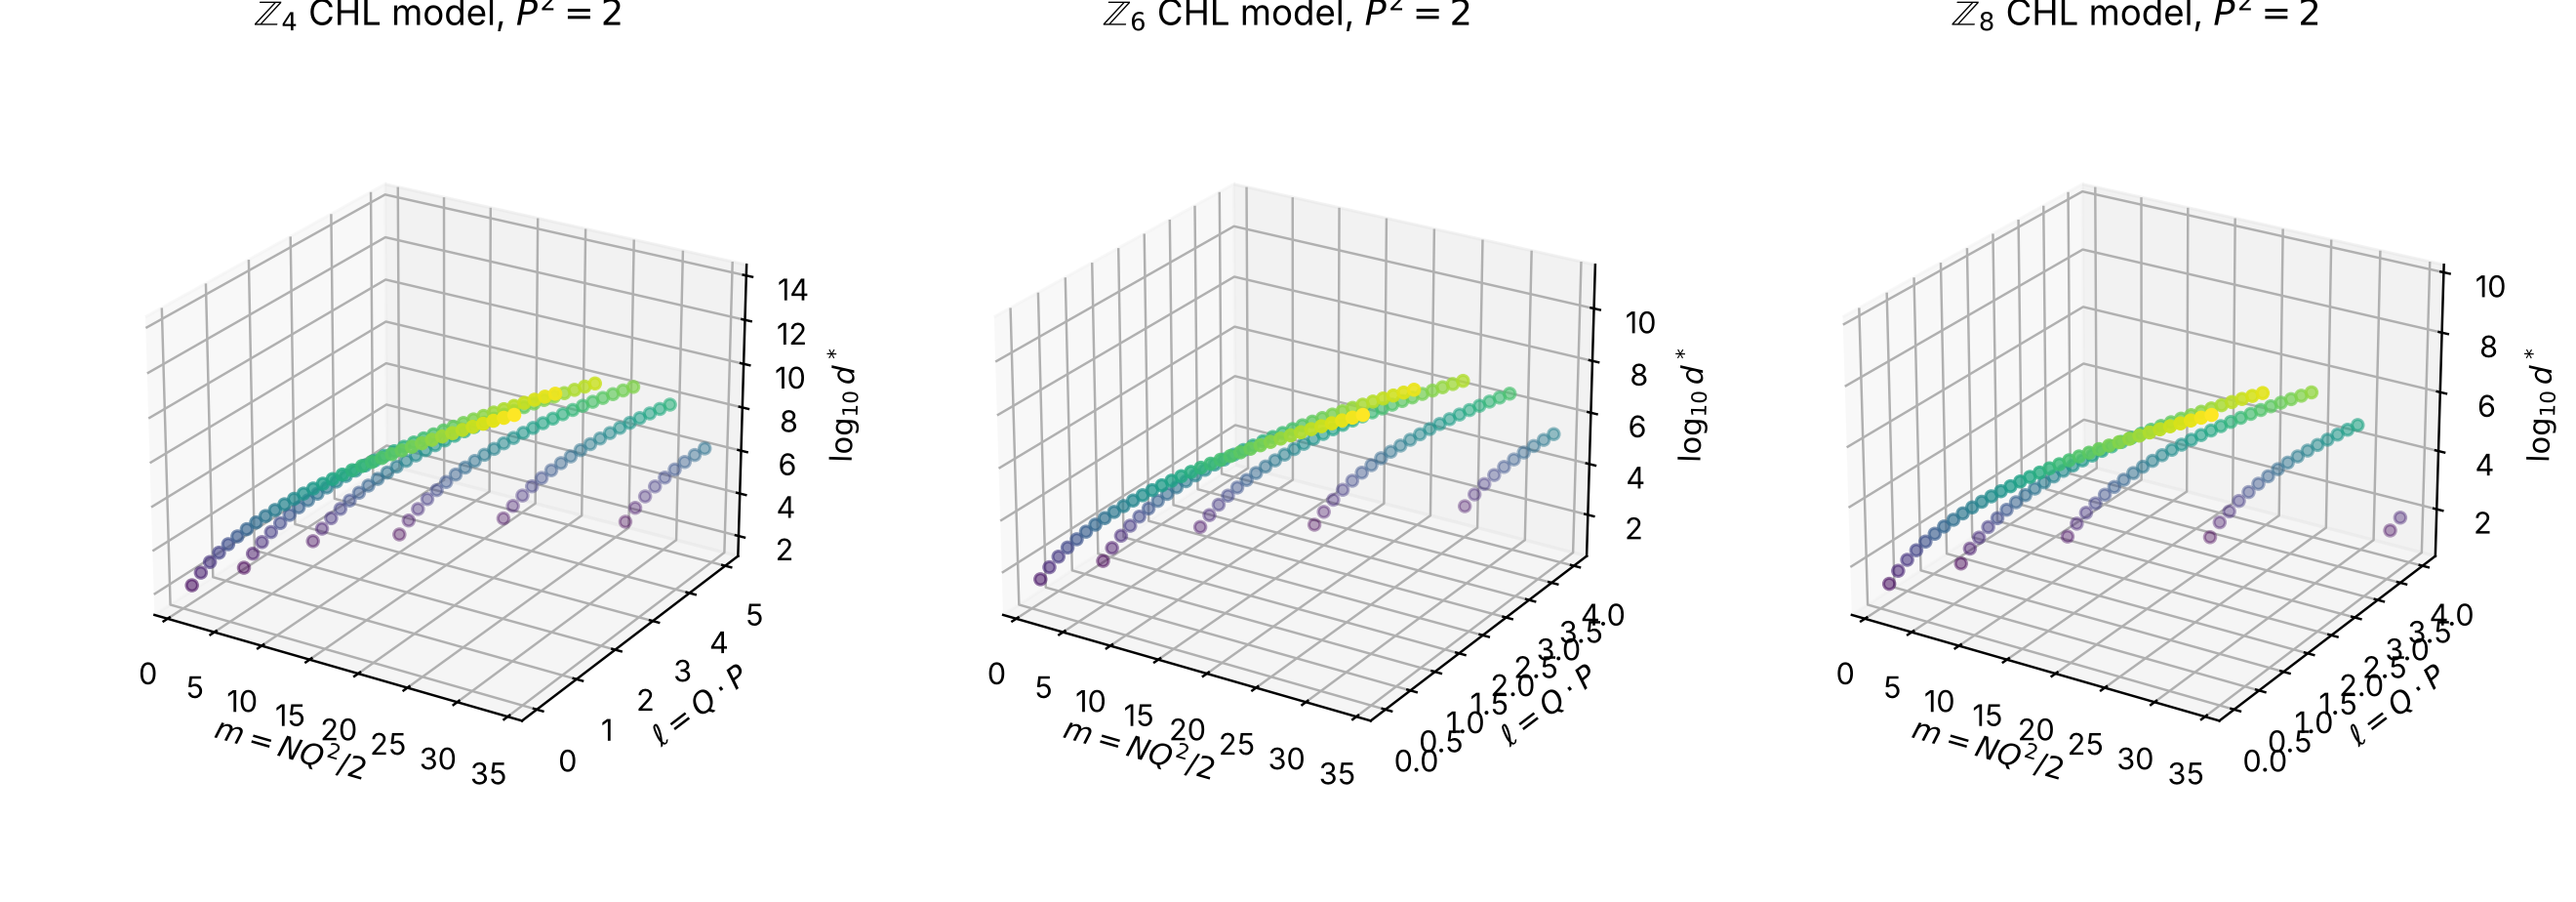
\includegraphics[width=\textwidth]{fig_index3d.png}
\caption{The single-centred index $d^*$ at $P^2=2$ for the CHL models of orders $4$, $6$ and $8$, plotted as $\log_{10}d^*$ against $m=NQ^2/2$ and $\ell=Q\cdot P\ge0$, for all charges with $\Delta>0$ and $m\le 34$. All values are positive, as Theorem~\ref{thm:A} asserts for every $m$.}
\label{fig:index}
\end{figure}

\subsection*{How the proof goes}
By the theorem of Bhand, Sen and Singh, at $P^2=2$ the index $d^*$ is, up to the sign $(-1)^{\ell+1}$, a Fourier coefficient of the finite part $\psi^F$ of the first Fourier--Jacobi coefficient $\psi_1$ of the partition function, taken in the variable conjugate to $P^2$ \cite[Theorem~5.4(b)]{BSS25}. The proof has four steps.

\begin{enumerate}
\item \emph{Closed form} (Theorem~\ref{thm:closed}). With $f$ the eta product of the cycle shape and $\gh=16,7,6$,
\[
f\,\psi^F=b\,\phi_{0,1}(N\tau,z)+c'\,\phi_{-2,1}(N\tau,z)-2\gh\,\Hc(N\tau,z),
\]
where $b$ and $c'$ are explicit modular forms of weight $2$ and $4$ for $\Gamma_0(N)$ and $\Hc$ is the generating function of Hurwitz class numbers. The proof uses only the modularity of $\psi_1$ and an identity of Bringmann and Murthy.
\item \emph{Theta decomposition} (Proposition~\ref{prop:coeff}). A short identity expressing $\phi_{0,1}$ through $\phi_{-2,1}$ and a theta quotient turns the closed form into two modular forms $G_0$, $G_1$ of weight $4$ for $\Gamma_0(4N)$, one for each parity of $\ell$; the index is a positive combination of their coefficients, corrected by a class number.
\item \emph{Positivity} (Proposition~\ref{prop:reps}). Each $G_\mu$ is a combination with nonnegative rational coefficients of products of theta series and Eisenstein series that have nonnegative coefficients. This settles all charges with $\ell$ even.
\item \emph{Domination} (Section~\ref{sec:proof}). For $\ell$ odd the class number enters with a negative sign. It grows at most linearly in $\Delta$, while the main term grows at least like $\Delta^5$; an explicit bound handles all large charges and an exact computation handles the rest.
\end{enumerate}

None of the steps uses an asymptotic formula, and no hypothesis is assumed. The computations used in the proof are finite, exact, and listed in Appendix~\ref{app:comp}.

\subsection*{Plan}
Section~\ref{sec:chl} recalls the CHL partition function and the definition of $d^*$. Section~\ref{sec:genera} expresses $\psi_1$ through twisted elliptic genera. Section~\ref{sec:closed} proves the closed form, Section~\ref{sec:theta} the theta decomposition and Section~\ref{sec:reps} the positivity of $G_0$ and $G_1$. Section~\ref{sec:proof} completes the proof and Section~\ref{sec:remarks} discusses what is not covered. Appendix~\ref{app:data} collects the data and Appendix~\ref{app:comp} the computations.

\subsection*{Notation}
Throughout, $\tau\in\HH$, $z\in\CC$, $\e(x)=e^{2\pi ix}$, $q=\e(\tau)$ and $\zeta=\e(z)$. For a series $F=\sum a(n)q^n$ we write $F(n)=a(n)$. Let $\eta(\tau)=q^{1/24}\prod_{n\ge1}(1-q^n)$ and let
\[
E_2=1-24\sum_{n\ge1}\sigma(n)q^n,\qquad E_4=1+240\sum_{n\ge1}\sigma_3(n)q^n,\]
\[\Ei(\tau)=2E_2(2\tau)-E_2(\tau)=1+24\sum_{n\ge1}\sigma^{\mathrm{odd}}(n)q^n,
\]
where $\sigma^{\mathrm{odd}}(n)$ is the sum of the odd divisors of $n$. The function $\Ei$ is a modular form of weight $2$ for $\Gamma_0(2)$ and spans $M_2(\Gamma_0(2))$ \cite{Ono04}. For $d\ge2$, $E_2(\tau)-dE_2(d\tau)\in M_2(\Gamma_0(d))$. We use the weak Jacobi forms of weight $-2$ and $0$ and index $1$ \cite[\S9]{EZ85},
\[
\phi_{-2,1}(\tau,z)=(\zeta-2+\zeta^{-1})\prod_{n\ge1}\frac{(1-q^n\zeta)^2(1-q^n\zeta^{-1})^2}{(1-q^n)^4},\qquad \phi_{0,1}(\tau,z)=(\zeta+10+\zeta^{-1})+O(q),
\]
normalised by $\phi_{0,1}(\tau,0)=12$, and write $c_{-2}(D)$ and $c_0(D)$ for their coefficients, which depend only on $D=4n-r^2$. The Hurwitz class number $H(D)$ is the number of $\mathrm{SL}_2(\ZZ)$-classes of positive definite binary quadratic forms of discriminant $-D$, the classes of $x^2+y^2$ and $x^2+xy+y^2$ counted with weights $\tfrac12$ and $\tfrac13$; we put $H(0)=-\tfrac1{12}$ and $H(D)=0$ for $D<0$ or $D\equiv1,2\pmod4$, and
\[
\Hc(\tau,z)=\sum_{n\ge0}\sum_{r\in\ZZ}H(4n-r^2)\,q^n\zeta^r .
\]
Finally $A_{1,1}(\tau,z)=\sum_{s\in\ZZ}q^{s^2+s}\zeta^{2s+1}(1-q^s\zeta)^{-2}$ is the Appell--Lerch sum of index $1$.

\section{The CHL models and the single-centred index}\label{sec:chl}

\subsection{Twisted elliptic genera}
Let $g$ be the generator of the orbifold group, of order $N$. For $r,s\in\ZZ/N\ZZ$ let
\[
F^{(r,s)}(\tau,z)=\frac1N\,\mathrm{Tr}_{\mathcal H_{g^r}}\Bigl(g^s(-1)^{F_L+F_R}q^{L_0-\frac c{24}}\bar q^{\bar L_0-\frac{\bar c}{24}}\zeta^{J_0}\Bigr)
\]
be the twisted elliptic genera of the $K3$ sigma model, the trace being over the Ramond--Ramond states twisted by $g^r$ \cite{DJS06,DJS07}. Write $F^{(r,s)}=\sum_{n\in\frac1N\ZZ,\,j\in\ZZ}c^{(r,s)}(4n-j^2)\,q^n\zeta^j$; the coefficient depends only on $4n-j^2$ and on $j\bmod2$, which we suppress. The untwisted sector gives the twining genera $NF^{(0,s)}=Z_{g^s}$, and for the classes that occur here
\begin{equation}\label{eq:twining}
Z_h(\tau,z)=\frac{\chi(h)}{12}\,\phi_{0,1}(\tau,z)+T_h(\tau)\,\phi_{-2,1}(\tau,z),
\end{equation}
where $\chi(h)$ is the number of fixed points of $h$ on $24$ letters and $T_h$ is the modular form of weight~$2$ in Table~\ref{tab:twining} \cite{Che10}. The twisted sectors follow from modular covariance: $F^{(r,s)}(\gamma\tau,\frac z{c\tau+d})\,\e(-\frac{cz^2}{c\tau+d})=F^{(ra+sc,\,rb+sd)}(\tau,z)$ for $\gamma=\left(\begin{smallmatrix}a&b\\c&d\end{smallmatrix}\right)\in\SL$ \cite{DJS07}. Hence $NF^{(r,s)}=\frac{\chi(g^d)}{12}\phi_{0,1}+(T_{g^d}|_2\gamma)\,\phi_{-2,1}$, where $d=\gcd(r,s,N)$ and $\gamma$ is any element of $\SL$ with $(0,d)\gamma\equiv(r,s)\pmod N$.\footnote{For the classes $2A$, $3A$, $4B$, $6A$, $8A$ the functions $T_h$ are modular for $\Gamma_0(o(h))$ without multiplier, so the result does not depend on the choice of $\gamma$.} The slash of the forms $\phi^{(M)}$ of Table~\ref{tab:twining} is explicit: if $\left(\begin{smallmatrix}Ma&Mb\\c&d\end{smallmatrix}\right)=\gamma'\left(\begin{smallmatrix}\alpha&\beta\\0&\delta\end{smallmatrix}\right)$ with $\gamma'\in\SL$ and $\alpha\delta=M$, then
\[
\phi^{(M)}|_2\gamma=\frac1{M-1}\Bigl(\frac M{\delta^2}E_2\Bigl(\frac{\alpha\tau+\beta}{\delta}\Bigr)-E_2(\tau)\Bigr),
\]
because the nonholomorphic corrections in the transformation of $E_2$ cancel. In particular every $T_{g^d}|_2\gamma$ is holomorphic on $\HH$ and has an expansion in nonnegative powers of $q^{1/N}$.

\begin{table}[t]
\centering
\caption{The functions $T_h$ of \eqref{eq:twining}, with $\phi^{(M)}=\frac{ME_2(M\tau)-E_2(\tau)}{M-1}\in M_2(\Gamma_0(M))$.}\label{tab:twining}
\begin{tabular}{llll}
\toprule
class & $\chi(h)$ & cycle shape & $T_h$\\
\midrule
$2A$ & $8$ & $1^82^8$ & $\frac43\phi^{(2)}$\\
$3A$ & $6$ & $1^63^6$ & $\frac32\phi^{(3)}$\\
$4B$ & $4$ & $1^42^24^4$ & $-\frac13\phi^{(2)}+2\phi^{(4)}$\\
$6A$ & $2$ & $1^22^23^26^2$ & $-\frac16\phi^{(2)}-\frac12\phi^{(3)}+\frac52\phi^{(6)}$\\
$8A$ & $2$ & $1^22\,4\,8^2$ & $-\frac12\phi^{(4)}+\frac73\phi^{(8)}$\\
\bottomrule
\end{tabular}
\end{table}

For $N=4$ the powers $g,g^2,g^3$ lie in $4B,2A,4B$; for $N=6$ the powers $g,\dots,g^5$ lie in $6A,3A,2A,3A,6A$; for $N=8$ the powers $g^d$ with $d=1,2,4$ lie in $8A,4B,2A$. The identity class has $\chi=24$ and $T=0$, so that $Z_1=2\phi_{0,1}$ is the elliptic genus of $K3$.

\subsection{The partition function}
The index of quarter-BPS dyons is generated by $1/\Phit$, where $\Phit$ is a Siegel modular form of weight $k=3,2,1$ for $N=4,6,8$ with the product expansion \cite{DJS06}, \cite[(5.2)]{BSS25}
\begin{equation}\label{eq:product}
\Phit(\tau,z,\sigma)=\e(\tau+z+\tfrac\sigma N)\prod_{r=0}^{N-1}\ \prod_{\substack{k'\in\ZZ+\frac rN,\ l\in\ZZ,\ j\in\ZZ\\ k',l\ge0,\ j<0\text{ if }k'=l=0}}\bigl(1-\e(k'\sigma+l\tau+jz)\bigr)^{a(k',l,j)},
\end{equation}
\[
a(k',l,j)=\sum_{s=0}^{N-1}\e\bigl(-\tfrac{sl}N\bigr)\,c^{(r,s)}(4k'l-j^2)\qquad(k'\in\ZZ+\tfrac rN).
\]
With the normalisation of $F^{(r,s)}$ used above the exponents $a(k',l,j)$ are integers.\footnote{As a check of the conventions, the same formula with $N=2$ and $N=3$ reproduces the indices $-B_6=2164$, $360$ at $(Q^2,P^2,Q\cdot P)=(1,2,0),(1,2,1)$ of \cite[Table~2]{Sen11} and $540$, $27$ at $(\frac23,2,0),(\frac23,2,1)$ of \cite[Table~3]{Sen11}; see Appendix~\ref{app:comp}.} For $\operatorname{Im}\sigma\to\infty$ there is an expansion \cite[Proposition~5.1]{BSS25}
\[
\frac1{\Phit(\tau,z,\sigma)}=\sum_{n\ge-1}\psi_n(\tau,z)\,\e\bigl(\tfrac{n\sigma}N\bigr),
\]
and $\psi_n$ is a meromorphic Jacobi form of weight $-k$ and index $n/N$ for $\Gamma_1(N)\ltimes(N\ZZ\times\ZZ)$ whose poles lie at $z\in N\ZZ\tau+\ZZ$ \cite[(5.39)]{BSS25}. The functions relevant to $P^2=2$ are $\psi_{-1}$ and $\psi_1$.

\subsection{The single-centred index}
The function $\psi_1$ has double poles at $z\in N\ZZ\tau+\ZZ$. Bhand, Sen and Singh split it as $\psi_1=\psi^P+\psi^F$ into a polar part \cite[(5.45)]{BSS25}
\begin{equation}\label{eq:polar}
\psi^P(\tau,z)=\frac{\gh}{f(\tau)}\,A_{1,1}(N\tau,z)=\frac{\gh}{f(\tau)}\sum_{s\in\ZZ}\frac{q^{N(s^2+s)}\zeta^{2s+1}}{(1-q^{Ns}\zeta)^2}
\end{equation}
and a finite part $\psi^F$, which is holomorphic in $z$; here $f$ and $\gh$ are given in Lemma~\ref{lem:psim1} and Lemma~\ref{lem:S} below.\footnote{In \cite{BSS25} the function $1/f$ is written $\tilde f^{(k)}(\tau)$ and $\gh$ is $\hat g^{(k)}(1)$, the coefficient of $\e(\sigma/N)$ in $1/g^{(k)}(\sigma/N)$. Both descriptions give the coefficient of the double pole of $\psi_1$ at $z=0$, which is what fixes $\psi^P$.} Write $\psi^F=\sum_{m,\ell}\cF(m,\ell)q^m\zeta^\ell$.

\begin{proposition}[Bhand--Sen--Singh]\label{prop:bss}
For every charge with $P^2=2$ and $\Delta>0$,
\[
d^*(Q,P)=(-1)^{\ell+1}\,\cF(m,\ell),\qquad m=\tfrac N2Q^2,\ \ell=Q\cdot P .
\]
\end{proposition}

\begin{proof}
By \cite[Theorem~5.4(b)]{BSS25} this holds for every triple $(n,\ell,m)$ in the set $B$ of \cite[(5.48)--(5.49)]{BSS25}, where $n=P^2/2$. For $n=1$ the defining condition of $B$ asks that $(n_1N\ell-2s-1)^2+n_1^2N(4m-N\ell^2)\ge1$ for all integers $n_1$ and $s$ (the congruence $s(s+1)\equiv0\pmod{n_1}$ there plays no role). If $n_1\ne0$ the second term is at least $N\Delta\ge N$, and if $n_1=0$ the first term is an odd square. So every charge with $P^2=2$ and $\Delta>0$ lies in $B$. The normalisation: the defining integral \cite[(5.13)]{BSS25} carries a factor $1/N$ and runs over $\operatorname{Re}\sigma\in[0,N)$; the $\sigma$-integral of $\e(n\sigma/N)\e(-n\sigma/N)$ over this interval equals $N$, and the two factors cancel. This agrees with the values of \cite[Tables~2--3]{Sen11} quoted above.
\end{proof}

So Theorem~\ref{thm:A} is equivalent to
\begin{equation}\label{eq:goal}
(-1)^{\ell+1}\cF(m,\ell)>0\qquad\text{whenever }4m-N\ell^2>0 .
\end{equation}
Integrality of $d^*$ is clear from \eqref{eq:product}, \eqref{eq:polar} and the integrality of the $a(k',l,j)$.

\section{The coefficient \texorpdfstring{$\psi_1$}{psi\_1} and the twisted genera}\label{sec:genera}

\begin{lemma}\label{lem:psim1}
Let $f$ be the eta product of the cycle shape of $g$:
\[
f=\eta(\tau)^4\eta(2\tau)^2\eta(4\tau)^4,\qquad \eta(\tau)^2\eta(2\tau)^2\eta(3\tau)^2\eta(6\tau)^2,\qquad \eta(\tau)^2\eta(2\tau)\eta(4\tau)\eta(8\tau)^2
\]
for $N=4,6,8$. Then $f\in M_{k+2}(\Gamma_0(N),\chi)$ with $\chi=\chi_{-4},\mathbf 1,\bigl(\frac{-2}\cdot\bigr)$ respectively, $\chi$ is trivial on $\Gamma_1(N)$, and
\[
\psi_{-1}(\tau,z)=\frac1{f(\tau)\,\phi_{-2,1}(N\tau,z)} .
\]
\end{lemma}

\begin{proof}
The modularity of $f$ and its character follow from the criterion for eta quotients \cite[Theorem~1.64]{Ono04}: in each case $\sum_\delta\delta r_\delta=24$, $\sum_\delta\frac N\delta r_\delta=24$, the weight is $\frac12\sum r_\delta=5,4,3=k+2$, and the character is $\bigl(\frac{(-1)^{k+2}\prod\delta^{r_\delta}}{\cdot}\bigr)$, which equals $\chi_{-4}$, $\mathbf 1$ and $\bigl(\frac{-2}\cdot\bigr)$; each of these is trivial on integers $d\equiv1\pmod N$.

The coefficient $\psi_{-1}$ is the reciprocal of the part of \eqref{eq:product} with $k'=0$. Since $c^{(0,s)}(D)=0$ for $D<-1$, only $j\in\{0,\pm1\}$ occur. From \eqref{eq:twining}, $c_0(-1)=c_{-2}(-1)=1$, $c_0(0)=10$, $c_{-2}(0)=-2$, and $T_h(0)=2-\chi(h)/12$ (because $Z_h$ has the coefficient $2$ at $\zeta^{\pm1}q^0$; indeed $\phi^{(M)}(0)=1$ and the coefficients in Table~\ref{tab:twining} sum to $2-\chi/12$), we get $Nc^{(0,s)}(-1)=2$ and $Nc^{(0,s)}(0)=\chi(g^s)-4$. Hence $a(0,l,\pm1)=2$ if $N\mid l$ and $0$ otherwise, and, writing the cycle shape as $\prod_aa^{m_a}$ so that $\chi(g^s)=\sum_{a\mid s}am_a$,
\[
a(0,l,0)=\frac1N\sum_{s=0}^{N-1}\e\bigl(-\tfrac{sl}N\bigr)\sum_{a\mid s}am_a-4[N\mid l]=\sum_{a:\ \frac Na\mid l}m_a-4[N\mid l].
\]
The cycle shapes are invariant under $a\mapsto N/a$, so $\prod_{l\ge1}(1-q^l)^{a(0,l,0)}=\prod_a\prod_{n\ge1}(1-q^{an})^{m_a}\cdot\prod_{n\ge1}(1-q^{Nn})^{-4}$. Together with the factor $\e(\tau+z)(1-\zeta^{-1})^2$ from $k'=l=0$, $j=-1$, and the factors $(1-q^{Nn}\zeta^{\pm1})^2$, this gives $q\prod_a\prod_n(1-q^{an})^{m_a}\cdot\phi_{-2,1}(N\tau,z)=f(\tau)\phi_{-2,1}(N\tau,z)$, since $\sum_a am_a=24$.
\end{proof}

Write $\e(\sigma/N)=p$. The factors of \eqref{eq:product} with $k'=\frac1N$ and $k'=\frac2N$ contribute, up to order $p^2$,
\[
\exp\Bigl(\sum_{l,j}a(\tfrac1N,l,j)\bigl(p\,q^l\zeta^j+\tfrac12p^2q^{2l}\zeta^{2j}\bigr)+\sum_{l,j}a(\tfrac2N,l,j)\,p^2q^l\zeta^j\Bigr),
\]
and the factors with $k'\ge\frac3N$ start at $p^3$. Therefore $\psi_1=\psi_{-1}S$ with
\begin{equation}\label{eq:S}
S=X_2+\tfrac12X_1^2,\qquad X_1=\sum_{l,j}a(\tfrac1N,l,j)q^l\zeta^j,\qquad X_2=\sum_{l,j}a(\tfrac2N,l,j)q^l\zeta^j+\tfrac12X_1(2\tau,2z).
\end{equation}

\begin{lemma}\label{lem:S}
In terms of the twisted genera,
\[
X_1=NF^{(1,0)}(N\tau,z),\qquad X_2=\frac12\sum_{s=0}^{N-1}\sum_{t=0}^1F^{(2,s)}\Bigl(\frac{N\tau+Nt-s}2,z\Bigr)+\frac N2F^{(1,0)}(2N\tau,2z).
\]
The function $S$ is entire in $z$, even in $z$, and $S(\tau,0)=\gh$ with
\[
\gh=\tfrac12\bigl(\chi(g)^2+2\chi(g)+\chi(g^2)\bigr)=16,\ 7,\ 6\qquad(N=4,6,8).
\]
\end{lemma}

\begin{proof}
For $k'=\frac1N$ the exponent $a(\frac1N,l,j)$ involves the coefficient of $q^{l/N}\zeta^j$ in $F^{(1,s)}$. Under $\tau\mapsto N\tau-s$ the term $q^n\zeta^j$ of $F^{(1,s)}$, $n\in\frac1N\ZZ$, becomes $\e(-sn)q^{Nn}\zeta^j$, which is the term $\e(-\frac{sl}N)q^l\zeta^j$ with $l=Nn$; so $X_1=\sum_sF^{(1,s)}(N\tau-s,z)$, and $F^{(1,s)}(\tau-s,z)=F^{(1,0)}(\tau,z)$ by modular covariance with $\gamma=\left(\begin{smallmatrix}1&-s\\0&1\end{smallmatrix}\right)$. For $k'=\frac2N$ only the terms $q^n\zeta^j$ of $F^{(2,s)}$ with $Nn$ even contribute, with $q^l=q^{Nn/2}$ and phase $\e(-sn/2)$; the average over $t\in\{0,1\}$ of the substitution $\tau\mapsto\frac{N\tau+Nt-s}2$ produces exactly these terms. This proves the formulas for $X_1$ and $X_2$. Each $F^{(r,s)}$ is entire and even in $z$, hence so is $S$. At $z=0$, $\phi_{-2,1}$ vanishes and $\phi_{0,1}=12$, so $NF^{(r,s)}(\tau,0)=\chi(g^{\gcd(r,s,N)})$. Hence $X_1(\tau,0)=\chi(g)$, the second part of $X_2(\tau,0)$ is $\frac12\chi(g)$, and the first part is $\frac1N\sum_s\chi(g^{\gcd(2,s,N)})=\frac12(\chi(g)+\chi(g^2))$, because $\gcd(2,s,N)$ is $2$ for even $s$ and $1$ for odd $s$. Adding up gives the formula for $\gh$, and the values follow from Table~\ref{tab:twining}.
\end{proof}

\begin{lemma}\label{lem:Smod}
Put $\Phi_0=\phi_{0,1}(N\tau,z)$ and $\Phi_2=\phi_{-2,1}(N\tau,z)$. Then $S$ is a holomorphic Jacobi form of weight $0$ and index $\frac2N$ for $\Gamma_1(N)\ltimes(N\ZZ\times\ZZ)$, and $\Phi_0,\Phi_2$ are weak Jacobi forms of weight $0,-2$ and index $\frac1N$ for $\Gamma_0(N)\ltimes(N\ZZ\times\ZZ)$. For every $\gamma\in\SL$ and every compact set $K\subset\CC$, the functions $S|_{0,2/N}\gamma$ and $\Phi_i|\gamma$ are bounded on $\{\operatorname{Im}\tau\ge1\}\times K$.
\end{lemma}

\begin{proof}
If $\phi$ is a Jacobi form of index $1$ for $\SL\ltimes\ZZ^2$, then $\phi(N\tau,z)$ transforms with index $\frac1N$ under $\Gamma_0(N)\ltimes(N\ZZ\times\ZZ)$; this is a direct computation; see \cite[\S4]{BSS25}. By Lemma~\ref{lem:psim1}, $S=\psi_1/\psi_{-1}=f\,\Phi_2\,\psi_1$, a product of a modular form of weight $k+2$ with character trivial on $\Gamma_1(N)$, a Jacobi form of weight $-2$ and index $\frac1N$, and a meromorphic Jacobi form of weight $-k$ and index $\frac1N$ for $\Gamma_1(N)\ltimes(N\ZZ\times\ZZ)$. This gives the transformation law; holomorphy follows from Lemma~\ref{lem:S}.

For the boundedness, write each term of $S$ in Lemma~\ref{lem:S} as $F^{(r,s)}(w,\lambda z)$ with $w=\frac{\alpha\tau+\beta}\delta$ and $\lambda\in\{1,2\}$, and $NF^{(r,s)}=\frac{\chi}{12}\phi_{0,1}+T\phi_{-2,1}$. For $\gamma\in\SL$ we have $\left(\begin{smallmatrix}\alpha&\beta\\0&\delta\end{smallmatrix}\right)\gamma=\gamma''\left(\begin{smallmatrix}\alpha'&\beta'\\0&\delta'\end{smallmatrix}\right)$ with $\gamma''\in\SL$ and $\alpha'\delta'=\alpha\delta$. Applying the transformation laws of $\phi_{0,1},\phi_{-2,1}$ under $\gamma''$ and the covariance of the $F^{(r,s)}$, the slash of each term by $\gamma$ becomes a term of the same kind, $F^{(r',s')}(w',\lambda'z)$ with $w'=\frac{\alpha'\tau+\beta'}{\delta'}$ and $\lambda'=\lambda\delta'/\delta$, the exponential factors cancelling because $S$ has the stated index. Each such term is a combination of $\phi_{0,1}(w',\lambda'z)$ and $\phi_{-2,1}(w',\lambda'z)$ with coefficients holomorphic at $\infty$ (Section~\ref{sec:chl}); as $\operatorname{Im}\tau\to\infty$ it tends, uniformly for $z\in K$, to a finite limit, because $\phi_{0,1}$ and $\phi_{-2,1}$ contain only nonnegative powers of $q$ and the coefficient of $q^n$ is a Laurent polynomial in $\zeta$ of degree at most $\sqrt{4n+1}$. The same argument applies to $\Phi_0$ and $\Phi_2$.
\end{proof}

\section{The finite part in closed form}\label{sec:closed}

\begin{proposition}\label{prop:structure}
There are $b\in M_2(\Gamma_1(N))$ and $c\in M_4(\Gamma_1(N))$ with
\[
S=\frac{\gh}{144}\,\Phi_0^2+\Phi_2\bigl(b\,\Phi_0+c\,\Phi_2\bigr).
\]
\end{proposition}

\begin{proof}
Let $R=S-\frac{\gh}{144}\Phi_0^2$. By Lemma~\ref{lem:S}, $R$ is even and vanishes at $z=0$, so it has a zero of order at least $2$ there. The elliptic transformations $z\mapsto z+\lambda N\tau+\mu$ multiply $R$ by a nowhere vanishing factor, so $R$ has a double zero at every point of $N\ZZ\tau+\ZZ$. The function $\phi_{-2,1}(\tau',z)=\vartheta_1(\tau',z)^2/\eta(\tau')^6$ has double zeros exactly at $z\in\ZZ+\ZZ\tau'$, because $\vartheta_1(\tau',\cdot)$ has simple zeros exactly there; so $\Phi_2$ has double zeros exactly on $N\ZZ\tau+\ZZ$. Hence $W=R/\Phi_2$ is entire in $z$, even, of weight $2$ and index $\frac1N$ for $\Gamma_1(N)\ltimes(N\ZZ\times\ZZ)$. Put $b(\tau)=W(\tau,0)/12$. The same argument applied to $W-b\Phi_0$ shows that $c=(W-b\Phi_0)/\Phi_2$ is entire in $z$, invariant under $z\mapsto z+N\tau$ and $z\mapsto z+1$, hence bounded in $z$ and therefore independent of $z$. The transformation law of $W$ under $\Gamma_1(N)$ at $z=0$ shows $b|_2\gamma=b$, and then $c|_4\gamma=c$.

It remains to see that $b$ and $c$ are holomorphic at every cusp. Fix $\gamma\in\SL$. By Lemma~\ref{lem:Smod}, $(R|\gamma)$ is bounded on $\{\operatorname{Im}\tau\ge1\}\times\{|z|=\rho\}$. The function $\Phi_2|\gamma$ is a nonzero multiple of $\phi_{-2,1}(w,\lambda z)$ for some $w=\frac{\alpha\tau+\beta}\delta$ and $\lambda>0$, and for $\rho$ small and $\operatorname{Im}\tau$ large it is bounded away from $0$ on $|z|=\rho$, since it tends to $\e(\lambda z)-2+\e(-\lambda z)$. Hence $W|\gamma$ is bounded on $|z|=\rho$, and by the maximum principle on $|z|\le\rho$; so $b|_2\gamma$ is bounded as $\operatorname{Im}\tau\to\infty$. The same argument gives the boundedness of $c|_4\gamma$.
\end{proof}

We now need the identity of Bringmann and Murthy \cite[\S3]{BM13}
\begin{equation}\label{eq:BM}
\frac{\phi_{0,1}(\tau,z)^2}{\phi_{-2,1}(\tau,z)}=144\,A_{1,1}(\tau,z)+E_4(\tau)\,\phi_{-2,1}(\tau,z)-288\,\Hc(\tau,z).
\end{equation}

\begin{theorem}\label{thm:closed}
Let $\Phi_0,\Phi_2$ be as in Lemma~\ref{lem:Smod} and write $\phi^{(d)}=\frac{dE_2(d\tau)-E_2(\tau)}{d-1}$. Then
\begin{equation}\label{eq:closed}
f\,\psi^F=b\,\Phi_0+c'\,\Phi_2-2\gh\,\Hc(N\tau,z),
\end{equation}
with $c'=c+\frac{\gh}{144}E_4(N\tau)$ and, for $N=4,6,8$ respectively,
\begin{align*}
b&=-\tfrac1{72}\phi^{(2)}-\tfrac5{24}\phi^{(4)}, & c'&=\tfrac1{120}E_4(\tau)-\tfrac7{360}E_4(2\tau)+\tfrac7{30}E_4(4\tau),\\
b&=-\tfrac1{288}\phi^{(2)}-\tfrac1{54}\phi^{(3)}-\tfrac{65}{864}\phi^{(6)}, & c'&=\tfrac7{3600}E_4(\tau)-\tfrac{29}{7200}E_4(2\tau)-\tfrac7{3600}E_4(3\tau)+\tfrac{81}{800}E_4(6\tau)\\
&&&\qquad+\tfrac15\,\eta(\tau)^2\eta(2\tau)^2\eta(3\tau)^2\eta(6\tau)^2,\\
b&=-\tfrac1{96}\phi^{(4)}-\tfrac7{96}\phi^{(8)}, & c'&=\tfrac7{11520}E_4(\tau)-\tfrac1{768}E_4(2\tau)+\tfrac1{1440}E_4(4\tau)+\tfrac1{12}E_4(8\tau)\\
&&&\qquad+\tfrac3{16}\,\eta(2\tau)^4\eta(4\tau)^4.
\end{align*}
\end{theorem}

\begin{proof}
By Lemma~\ref{lem:psim1} and Proposition~\ref{prop:structure},
\[
f\psi_1=\frac{S}{\Phi_2}=\frac{\gh}{144}\frac{\Phi_0^2}{\Phi_2}+b\Phi_0+c\Phi_2 .
\]
Substituting \eqref{eq:BM} at $N\tau$ gives $f\psi_1=\gh A_{1,1}(N\tau,z)+b\Phi_0+c'\Phi_2-2\gh\Hc(N\tau,z)$, and the first term is $f\psi^P$ by \eqref{eq:polar}. This proves \eqref{eq:closed} with $b$, $c$ from Proposition~\ref{prop:structure}. The stated expressions are modular forms for $\Gamma_0(N)\subset\Gamma_1(N)$ of the right weight: $\phi^{(d)}\in M_2(\Gamma_0(d))$, $E_4(d\tau)\in M_4(\Gamma_0(d))$, and the two eta products are cusp forms of weight $4$ for $\Gamma_0(6)$ and $\Gamma_0(8)$ by \cite[Theorem~1.64]{Ono04}. By Sturm's theorem \cite{Stu87} a form of weight $w$ for $\Gamma_1(N)$ is determined by its coefficients up to $q^{\lfloor w\mu/12\rfloor}$, where $\mu=[\SL:\Gamma_1(N)]=12,24,48$. These bounds are $2,4,8$ for $b$ and $4,8,16$ for $c'$. We computed the coefficients of $S$, hence of $b$ and $c'$, through $q^{39}$ from the twisted genera of Section~\ref{sec:chl} (Appendix~\ref{app:comp}), and they agree with the stated expressions.
\end{proof}

In terms of the forms $E_2(\tau)-dE_2(d\tau)$ of $M_2(\Gamma_0(d))$ the coefficients $b$ read
\begin{align*}
N=4:&\quad b=\tfrac1{72}\bigl(E_2-2E_2(2\tau)\bigr)+\tfrac5{72}\bigl(E_2-4E_2(4\tau)\bigr),\\
N=6:&\quad b=\tfrac1{288}\bigl(E_2-2E_2(2\tau)\bigr)+\tfrac1{108}\bigl(E_2-3E_2(3\tau)\bigr)+\tfrac{13}{864}\bigl(E_2-6E_2(6\tau)\bigr),\\
N=8:&\quad b=\tfrac1{288}\bigl(E_2-4E_2(4\tau)\bigr)+\tfrac1{96}\bigl(E_2-8E_2(8\tau)\bigr).
\end{align*} Their constant terms are $b(0)=-\frac29,-\frac7{72},-\frac1{12}$, and $b(0)+c'(0)=0$ in all three cases.

\section{Theta decomposition}\label{sec:theta}

Let $\vartheta_2(\tau,z)=\sum_{n\in\ZZ}q^{(n+\frac12)^2/2}\zeta^{n+\frac12}$ and $\vartheta_2(\tau)=\vartheta_2(\tau,0)$, and let $\theta(\tau)=\sum_{n\in\ZZ}q^{n^2}$ and $\theta_4(\tau)=\theta(\tau+\frac12)=\sum_n(-1)^nq^{n^2}$. For $\mu\in\{0,1\}$ put
\[
\vtn_\mu(\tau)=\sum_{u\in\ZZ,\ u\not\equiv\mu\ (2)}q^{u^2/4},\qquad\text{so that}\quad \vtn_1=\theta,\quad \vtn_0=2q^{1/4}\sum_{v\ge0}q^{v(v+1)}.
\]

\begin{lemma}\label{lem:theta}
$\phi_{0,1}(\tau,z)=12\,\vartheta_2(\tau,z)^2/\vartheta_2(\tau)^2-2\,\Ei(\tau)\,\phi_{-2,1}(\tau,z)$. Consequently, for every $\ell\in\ZZ$ with $\mu\equiv\ell\pmod 2$,
\begin{align*}
\sum_{n}c_{-2}(4n-\ell^2)\,q^{n-\ell^2/4}&=(-1)^{\ell+1}\,\frac{\vtn_\mu(\tau)}{\eta(\tau)^6},\\
\sum_{n}c_{0}(4n-\ell^2)\,q^{n-\ell^2/4}&=\frac{\vtn_\mu(\tau)}{\eta(\tau)^6}\Bigl(3\theta_4(\tau)^4+2(-1)^\ell\,\Ei(\tau)\Bigr).
\end{align*}
\end{lemma}

\begin{proof}
Let $J=12\vartheta_2(\tau,z)^2/\vartheta_2(\tau)^2-\phi_{0,1}$. Since $\vartheta_2(\tau)=2\eta(2\tau)^2/\eta(\tau)$ is a modular form of weight $\frac12$ for $\Gamma_0(2)$ with a multiplier, and $\vartheta_2(\tau,z)$ transforms under $\Gamma_0(2)$ with the same multiplier and the factor of a Jacobi form of index $\frac12$, the quotient $\vartheta_2(\tau,z)^2/\vartheta_2(\tau)^2$ is a Jacobi form of weight $0$ and index $1$ for $\Gamma_0(2)\ltimes\ZZ^2$. It has nonnegative powers of $q$ at both cusps of $\Gamma_0(2)$: at $\infty$ it equals $\frac14(\zeta+2+\zeta^{-1})+O(q)$, and at $0$ it becomes $\vartheta_4(\tau,z)^2/\vartheta_4(\tau)^2=1+O(q^{1/2})$. So $J$ is a weak Jacobi form of weight $0$ and index $1$ for $\Gamma_0(2)$, even in $z$, with $J(\tau,0)=0$. As in the proof of Proposition~\ref{prop:structure}, $J/\phi_{-2,1}$ is a holomorphic modular form of weight $2$ for $\Gamma_0(2)$, hence a multiple of $\Ei$. Its constant term is found from $J=3\zeta+6+3\zeta^{-1}-(\zeta+10+\zeta^{-1})+O(q)=2(\zeta-2+\zeta^{-1})+O(q)$, so $J=2\Ei\,\phi_{-2,1}$.

For the coefficients, $\vartheta_2(\tau,z)^2=\sum_{a,b}q^{((a+\frac12)^2+(b+\frac12)^2)/2}\zeta^{a+b+1}$; with $\ell=a+b+1$ and $u=a-b$ the exponent is $(\ell^2+u^2)/4$ and $u\not\equiv\ell\pmod2$. Hence $\vartheta_2(\tau,z)^2=\sum_\ell\zeta^\ell q^{\ell^2/4}\vtn_\ell$. In the same way $\phi_{-2,1}=\vartheta_1(\tau,z)^2/\eta^6$ with $\vartheta_1(\tau,z)=\sum_n(-1)^nq^{(n+\frac12)^2/2}\zeta^{n+\frac12}$ gives the first formula. For the second, the eta quotients $\vartheta_2(\tau)=2\eta(2\tau)^2/\eta(\tau)$ and $\theta_4(\tau)=\eta(\tau)^2/\eta(2\tau)$ \cite{Ono04} give $12\eta(\tau)^6/\vartheta_2(\tau)^2=3\theta_4(\tau)^4$, and the formula follows from the first part.
\end{proof}

For $\mu\in\{0,1\}$ define the modular forms of weight $4$
\begin{equation}\label{eq:Gmu}
G_\mu=(-1)^{\mu+1}\,3\,b\,\theta_4(N\tau)^4+c'-2b\,\Ei(N\tau)\in M_4(\Gamma_0(4N)),
\end{equation}
which lie in $M_4(\Gamma_0(4N))$ because $\theta_4^4=\eta(\tau)^8/\eta(2\tau)^4\in M_2(\Gamma_0(4))$, and let
\[
\mathbb E_\mu(\tau)=\frac{\vtn_\mu(N\tau)}{\eta(N\tau)^6}\,G_\mu(\tau),\qquad \mathbb E_\mu(\Delta)=\text{the coefficient of }q^{\Delta/4}\text{ in }\mathbb E_\mu .
\]
Let $1/f=q^{-1}\sum_{i\ge0}p_N(i)q^i$. Since $1/f=q^{-1}\prod_a\prod_n(1-q^{an})^{-m_a}$ with all $m_a\ge0$, every $p_N(i)$ is a positive integer, and $p_N(0)=1$.

\begin{proposition}\label{prop:coeff}
For integers $m,\ell$ with $\mu\equiv\ell\pmod2$ and $\Delta=4m-N\ell^2$, put
\[
\mathcal P(m,\ell)=\mathbb E_\mu(\Delta)+(-1)^\mu\,2\gh\,h_N(m,\ell),\qquad h_N(m,\ell)=\begin{cases}H\bigl(\tfrac{4m}N-\ell^2\bigr)&N\mid m,\\0&N\nmid m.\end{cases}
\]
Then $(-1)^{\ell+1}$ times the coefficient of $q^m\zeta^\ell$ in $f\psi^F$ is $\mathcal P(m,\ell)$, and
\[
(-1)^{\ell+1}\cF(m,\ell)=\sum_{i\ge0}p_N(i)\,\mathcal P(m+1-i,\ell).
\]
\end{proposition}

\begin{proof}
Apply Lemma~\ref{lem:theta} at $(N\tau,z)$ to $b\Phi_0+c'\Phi_2$. The coefficient of $\zeta^\ell$ is
\[
q^{N\ell^2/4}\frac{\vtn_\mu(N\tau)}{\eta(N\tau)^6}\Bigl(b\bigl(3\theta_4(N\tau)^4+2(-1)^\ell\Ei(N\tau)\bigr)+(-1)^{\ell+1}c'\Bigr)=(-1)^{\ell+1}q^{N\ell^2/4}\,\mathbb E_\mu(\tau),
\]
because $(-1)^{\ell+1}\bigl(3b\theta_4^4(N\tau)+2(-1)^\ell b\Ei(N\tau)\bigr)+c'=G_\mu$. The coefficient of $q^m$ is $(-1)^{\ell+1}\mathbb E_\mu(\Delta)$. The term $-2\gh\Hc(N\tau,z)$ contributes $-2\gh H(4n-\ell^2)$ at $q^{Nn}\zeta^\ell$ and nothing at $q^m$ with $N\nmid m$; multiplying by $(-1)^{\ell+1}$ gives $(-1)^\mu2\gh h_N(m,\ell)$. The last formula follows from $\psi^F=f^{-1}\cdot f\psi^F$.
\end{proof}

\begin{lemma}\label{lem:small}
$\mathcal P(m,\ell)=0$ if $\Delta\le0$.
\end{lemma}

\begin{proof}
Assume $\Delta\le 0$. First let $\mu=0$. Then $\mathbb E_0=2\sum_{v\ge0}q^{Nv(v+1)}\prod_n(1-q^{Nn})^{-6}\cdot G_0$ is a power series in $q$ with constant term $2G_0(0)$, so $\mathbb E_0(\Delta)=0$ for $\Delta<0$. If $\Delta=0$, then $\ell$ is even, $4m=N\ell^2$, $N\mid m$ and $h_N=H(0)=-\frac1{12}$, so $\mathcal P(m,\ell)=2G_0(0)-\frac{\gh}6$. Now $G_0(0)=c'(0)-5b(0)=-6b(0)$, because $b(0)+c'(0)=0$, and this equals $\frac43,\frac7{12},\frac12$, which is $\gh/12$ in each case. Hence $\mathcal P=0$. Next let $\mu=1$. Then $\mathbb E_1=q^{-N/4}\theta(N\tau)\prod_n(1-q^{Nn})^{-6}\,G_1$, and $G_1=O(q^{m_N})$ with $m_N=2,2,3$ (Proposition~\ref{prop:reps}), so $\mathbb E_1=O(q^{m_N-N/4})$ with $m_N-\frac N4>0$; thus $\mathbb E_1(\Delta)=0$ for $\Delta\le0$. Finally $h_N(m,\ell)=0$ for $\Delta<0$, and for $\Delta=0$ with $\ell$ odd we have $N\ell^2=4m$, which forces $\ell$ even when $N=6$, and $m\equiv\frac N4\pmod N$ when $N=4,8$; in either case $h_N=0$.
\end{proof}

\section{Positivity of \texorpdfstring{$G_0$}{G\_0} and \texorpdfstring{$G_1$}{G\_1}}\label{sec:reps}

We use the following building blocks, all of which have nonnegative Fourier coefficients:
\[
t_a=\theta(a\tau)^2,\qquad s_a=\frac{\eta(8a\tau)^4}{\eta(4a\tau)^2}=q^a\Bigl(\sum_{n\ge0}q^{2an(n+1)}\Bigr)^2,\qquad e_d=\Ei(d\tau),\qquad E_4(d\tau).
\]

\begin{lemma}\label{lem:blocks}
$t_a\in M_1(\Gamma_0(4a),\chi_{-4})$, $s_a\in M_1(\Gamma_0(8a),\chi_{-4})$, $e_d\in M_2(\Gamma_0(2d))$ and $E_4(d\tau)\in M_4(\Gamma_0(d))$. The coefficients of $t_a$ and $s_a$ are nonnegative integers, those of $e_d$ and $E_4(d\tau)$ positive at every multiple of $d$, and $t_1^2=\theta^4$ has a positive coefficient at every $n\ge0$.
\end{lemma}

\begin{proof}
For $t_a$ this is the classical fact $\theta^2\in M_1(\Gamma_0(4),\chi_{-4})$. For $s_a$: Gauss's identity $\sum_{n\ge0}x^{n(n+1)/2}=\prod_{n\ge1}(1-x^{2n})^2/(1-x^n)$ at $x=q^{4a}$ gives the product form, and the eta quotient criterion \cite[Theorem~1.64]{Ono04} with $\sum\delta r_\delta=24a$, $\sum\frac{8a}\delta r_\delta=0$ and character $\bigl(\frac{-256}\cdot\bigr)=\chi_{-4}$ gives the modularity; holomorphy at the cusps follows from \cite[Theorem~1.65]{Ono04}. The statements on $e_d$ and $E_4$ are clear. Finally $\theta^4(n)=r_4(n)>0$ by Lagrange's four squares theorem.
\end{proof}

\begin{proposition}\label{prop:reps}
For each $N\in\{4,6,8\}$ and $\mu\in\{0,1\}$, $G_\mu$ equals the combination with nonnegative rational coefficients of products of building blocks given in Appendix~\ref{app:data}. In particular:
\begin{enumerate}
\item $G_0(n)>0$ for all $n\ge0$;
\item $G_1(n)=0$ for $n<m_N$ and $G_1(n)>0$ for $n\ge m_N$, where $m_N=2,2,3$;
\item $G_1(n)\ge0$ for all $n$, and $\gamma_N=\min\{G_1(n):m_N\le n<m_N+N\}=8,1,2$.
\end{enumerate}
\end{proposition}

\begin{proof}
Each product in Appendix~\ref{app:data} is a form of weight $4$ for $\Gamma_0(4N)$ with trivial character, by Lemma~\ref{lem:blocks}: every factor has level dividing $4N$, and the characters $\chi_{-4}$ occur an even number of times. By Sturm's theorem a form of weight $4$ for $\Gamma_0(L)$ is determined by its coefficients up to $q^{\lfloor[\SL:\Gamma_0(L)]/3\rfloor}$; for $L=16,24,32$ the index is $24,48,48$ and the bound is $8,16,16$. Both sides were computed through $q^{100}$ and agree (Appendix~\ref{app:comp}). Nonnegativity of all coefficients follows from Lemma~\ref{lem:blocks}.

(1) The representation of $G_0$ contains $e_1e_2$ (for $N=4,8$) or $e_1e_3$ (for $N=6$) with positive coefficient, and $e_1$ has a positive coefficient at every $n\ge0$ while the second factor has constant term $1$.

(2) Every product in the representation of $G_1$ contains a factor $s_2$ ($N=4$), $s_1^2$ or $s_3$ ($N=6$), or $s_4$ or $s_1s_2$ ($N=8$), and these are $O(q^{m_N})$. For positivity at $n\ge m_N$: when $N=4$, the term $\frac13t_2s_2e_1$ has coefficient at least $\frac13$ at each $n\ge2$ because $e_1(j)\ge1$ for all $j$; when $N=6$, the term $\frac{265}{9558}t_1s_3e_1$ covers $n\ge3$ and $\frac{448}{531}t_1t_3s_1^2$ covers $n=2$; when $N=8$, the term $t_1^2t_4s_4$ covers $n\ge4$ by Lagrange's theorem and $t_1t_4s_1s_2$ covers $n=3$.

(3) The values of $G_1$ on the window are listed in Table~\ref{tab:G}.
\end{proof}

\begin{figure}[t]
\centering
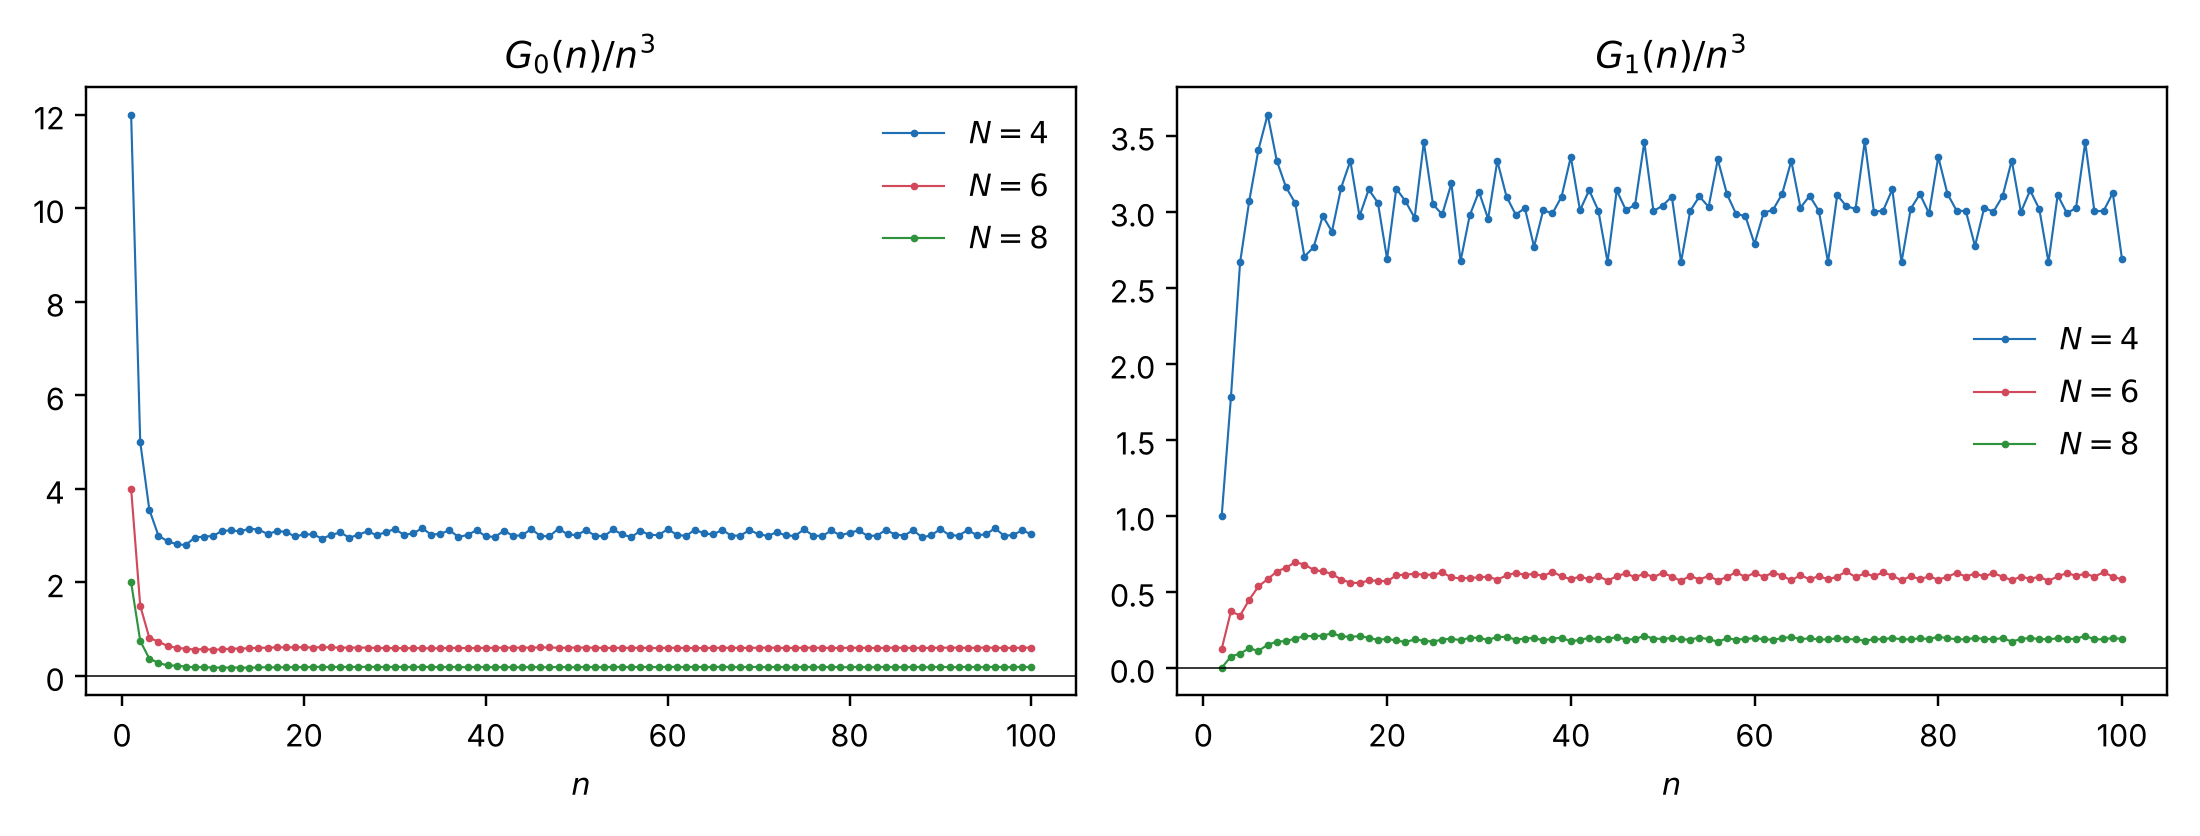
\includegraphics[width=\textwidth]{fig_Gmu.png}
\caption{The normalised coefficients $G_0(n)/n^3$ and $G_1(n)/n^3$ for $n\le100$. Both forms have nonnegative coefficients (Proposition~\ref{prop:reps}) and grow like $n^3$, as Eisenstein series of weight $4$ do.}
\label{fig:G}
\end{figure}

\section{Proof of Theorem~\ref{thm:A}}\label{sec:proof}

By Proposition~\ref{prop:bss} and Proposition~\ref{prop:coeff} it suffices to show that
\begin{equation}\label{eq:Ppos}
\mathcal P(m,\ell)\ge0\ \text{ for all }m,\ell,\qquad \mathcal P(m,\ell)>0\ \text{ when }4m-N\ell^2>0 .
\end{equation}
Indeed, if $\Delta=4m-N\ell^2>0$, then all terms of the sum in Proposition~\ref{prop:coeff} are nonnegative and the term $i=0$ is $\mathcal P(m+1,\ell)>0$, since $4(m+1)-N\ell^2=\Delta+4>0$; so $(-1)^{\ell+1}\cF(m,\ell)>0$. By Lemma~\ref{lem:small} we may assume $\Delta>0$.

\subsection*{Even \texorpdfstring{$\ell$}{l}} Then $\mu=0$, $4\mid\Delta$ and $(-1)^\mu2\gh h_N\ge0$. The series $\vtn_0(N\tau)/\eta(N\tau)^6=2\sum_{v\ge0}q^{Nv(v+1)}\prod_n(1-q^{Nn})^{-6}$ has nonnegative coefficients and constant term $2$, so $\mathcal P(m,\ell)\ge\mathbb E_0(\Delta)\ge2G_0(\Delta/4)>0$ by Proposition~\ref{prop:reps}(1).

\subsection*{Odd \texorpdfstring{$\ell$}{l}} Then $\mu=1$ and
\[
\mathbb E_1(\Delta)=\sum_{j\ge0}a_j\,G_1(n-Nj),\qquad n=\frac{\Delta+N}4=m-N\frac{\ell^2-1}4,
\]
where $a_j$ are the coefficients of $\theta(\tau)\prod_{k\ge1}(1-q^k)^{-6}$. Note that $n$ is an integer, $n\equiv m\pmod N$ (because $8\mid\ell^2-1$), and $n\ge m_N$ because $\Delta>0$ means $4n>N$ and $n\ge2,2,3$ follows for $N=4,6,8$. All $a_j$ are positive integers, and comparing with $(1-q)^{-6}$ gives $a_j\ge\binom{j+5}5$. If $N\nmid m$, then $h_N=0$ and $\mathcal P(m,\ell)\ge a_0G_1(n)>0$ by Proposition~\ref{prop:reps}(2). If $N\mid m$, then $N\mid n$ and
\[
\mathcal P(m,\ell)=\mathbb E_1(\Delta)-2\gh\,H(D),\qquad D=\frac\Delta N=\frac{4n}N-1\ge3 .
\]

\begin{lemma}\label{lem:H}
$H(D)\le D$ for every integer $D\ge1$.
\end{lemma}

\begin{proof}
Every class contains a reduced form $[a,b,c]$ with $|b|\le a\le c$ and $4ac-b^2=D$, so $3a^2\le D$. For each $a\le A=\lfloor\sqrt{D/3}\rfloor$ there are at most $a+1$ values of $b$ with $|b|\le a$ and $b\equiv D\pmod2$, and $b$ determines $c$. Hence $H(D)\le\sum_{a=1}^A(a+1)=\frac{A(A+3)}2\le\frac{D/3+3\sqrt{D/3}}2$, which is at most $D$ when $3\sqrt{D/3}\le\frac53D$, that is, for $D\ge\frac{27}{25}$. For $D=1$ there is no form and $H(1)=0$.
\end{proof}

Let $J=\lfloor(n-m_N)/N\rfloor$, so that $n-NJ$ lies in the window $[m_N,m_N+N)$ of Proposition~\ref{prop:reps}(3). Keeping only the term $j=J$,
\begin{equation}\label{eq:lower}
\mathbb E_1(\Delta)\ge\binom{J+5}5\gamma_N,\qquad 2\gh H(D)\le2\gh D<\frac{8\gh n}N .
\end{equation}

\emph{Large $n$.} Since $\binom{J+5}5\ge\frac{(J+1)^2}2$ and $J+1\ge\frac{n-m_N+1}N\ge\frac n{2N}$ for $n\ge2m_N$, the right side of the first inequality is at least $\gamma_Nn^2/(8N^2)$, which exceeds $8\gh n/N$ as soon as
\[
n>n_N=\frac{64\gh N}{\gamma_N}=512,\ 2688,\ 1536\qquad(N=4,6,8).
\]

\emph{Moderate $n$.} For $60\le n\le3000$ the inequality $\binom{J+5}5\gamma_N>8\gh n/N$ was checked directly; it holds from $n=18,38,43$ on for $N=4,6,8$.

\emph{Small $n$.} For $m_N\le n<60$ with $N\mid n$ the exact values of $\mathbb E_1(\Delta)$ and $H(D)$ were computed, and $\mathbb E_1(\Delta)>2\gh H(D)$ in every case.

This proves \eqref{eq:Ppos} and hence Theorem~\ref{thm:A}. \qed

\begin{figure}[t]
\centering
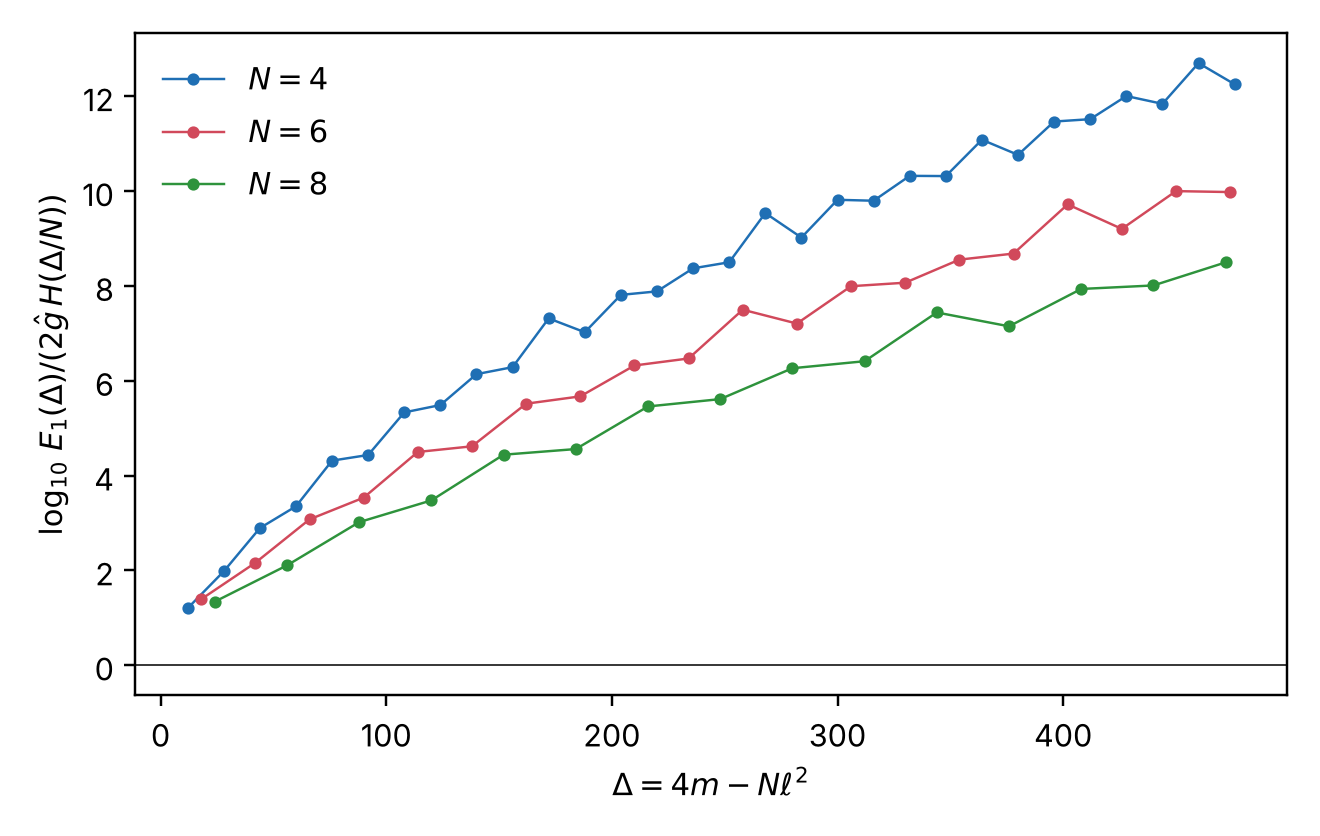
\includegraphics[width=0.62\textwidth]{fig_margin.png}
\caption{The margin $\log_{10}\bigl(\mathbb E_1(\Delta)/2\gh H(\Delta/N)\bigr)$ for the charges with $\ell$ odd and $N\mid m$, the only ones in which the class number is subtracted. The ratio is smallest at the first charge and grows rapidly with $\Delta$.}
\label{fig:margin}
\end{figure}

\section{Remarks}\label{sec:remarks}

\subsection*{What the proof covers}
Theorem~\ref{thm:A} concerns $P^2=2$, the first Fourier--Jacobi coefficient in the variable conjugate to $P^2$. By the S-duality invariance $d^*(Q,P)=d^*(Q',P')$ under $\Gamma_1(N)$ \cite[(5.18)]{BSS25} it extends to every charge in the $\Gamma_1(N)$-orbit of a charge with $P^2=2$, but it does not give the sign for general $(Q^2,P^2)$. For larger $P^2$ the polar part of $\psi_n$ involves Appell--Lerch sums of higher index and the closed form contains Hecke-type images of $\Hc$ whose coefficients are not single class numbers; the method extends in principle, but the representations of Section~\ref{sec:reps} would have to be found anew for each $n$.

\subsection*{Where the proof is tight}
The positivity for even $\ell$ holds with room to spare: the class number then enters with a positive sign. For odd $\ell$ the binding cases are the smallest charges with $N\mid m$; at $N=6$, $m=6$, $\ell=1$ one has $\Delta=18$, $\mathbb E_1(18)=G_1(6)=\frac{347}3$ and $2\gh H(3)=\frac{14}3$. The window minimum $\gamma_6=1$ is attained at $n=2$, where $G_1(2)=1$ comes from the two terms $\frac{448}{531}t_1t_3s_1^2$ and $\frac{83}{531}s_1^2e_1$.

\subsection*{Toroidal models}
Chattopadhyaya and David found that positivity fails for some single-centred dyons in the $\ZZ_2$ and $\ZZ_3$ orbifolds of type~II string theory on $T^6$ \cite{CD19}, and interpreted this as a sign of nontrivial hair; see also \cite{CD21}. Theorem~\ref{thm:A} shows that no such failure occurs at $P^2=2$ for the composite $K3$ orbifolds.

\subsection*{Duality frames}
The CHL models are dual to heterotic string theory on $T^6$ divided by a $\ZZ_N$ symmetry \cite{CHL95}; for the role of heterotic compactifications in eleven-dimensional supergravity see \cite{SBBT26}. The charges $Q,P$ and the index $d^*$ are frame independent.

\appendix

\section{Data}\label{app:data}

\subsection*{The representations of \texorpdfstring{$G_\mu$}{G\_mu}}
With $t_a,s_a,e_d$ as in Section~\ref{sec:reps}:

\noindent$N=4$:
\begin{align*}
G_0&=\tfrac{3}{160}\,t_{1}^{4} + \tfrac{1}{8}\,t_{2}^{2}e_{1} + \tfrac{5}{6}\,t_{2}t_{4}e_{2} + \tfrac{1}{45}\,e_{1}e_{2} + \tfrac{1}{3}\,e_{1}e_{8} + \tfrac{1}{1440}\,E_4(\tau),\\
G_1&=5\,t_{1}^{2}t_{2}s_{2} + \tfrac{8}{3}\,t_{2}^{2}t_{4}s_{2} + \tfrac{1}{3}\,t_{2}s_{2}e_{1}.
\end{align*}
$N=6$:
\begin{align*}
G_0&=\tfrac{1009}{38448}\,t_{1}^{2}t_{2}^{2} + \tfrac{3715}{153792}\,t_{1}^{2}t_{3}^{2} + \tfrac{215}{12816}\,t_{1}^{2}e_{3} + \tfrac{17}{6408}\,t_{1}^{2}e_{4} + \tfrac{167}{712}\,t_{1}t_{6}^{3} + \tfrac{4769}{115344}\,t_{1}t_{6}e_{1}\\
&\quad + \tfrac{269}{14418}\,t_{1}t_{6}e_{4} + \tfrac{220}{7209}\,t_{2}^{2}e_{12} + \tfrac{919}{12816}\,t_{2}t_{3}e_{2} + \tfrac{17}{712}\,t_{3}^{2}e_{12} + \tfrac{407}{461376}\,e_{1}e_{3} + \tfrac{1001}{19224}\,e_{1}e_{12}\\
&\quad + \tfrac{2011}{173016}\,e_{2}e_{6} + \tfrac{415}{57672}\,e_{2}e_{12} + \tfrac{3647}{173016}\,e_{4}e_{6},\\
G_1&=\tfrac{448}{531}\,t_{1}t_{3}s_{1}^{2} + \tfrac{265}{9558}\,t_{1}s_{3}e_{1} + \tfrac{532}{4779}\,t_{1}s_{3}e_{2} + \tfrac{151}{531}\,t_{1}s_{3}e_{3} + \tfrac{361}{531}\,t_{1}s_{3}e_{6} + \tfrac{415}{6372}\,t_{2}s_{3}e_{1}\\
&\quad + \tfrac{421}{2124}\,t_{2}s_{3}e_{3} + \tfrac{2147}{6372}\,t_{3}s_{3}e_{1} + \tfrac{2191}{3186}\,t_{3}s_{3}e_{2} + \tfrac{86}{531}\,t_{3}s_{3}e_{4} + \tfrac{227}{708}\,t_{6}s_{3}e_{3} + \tfrac{83}{531}\,s_{1}^{2}e_{1}\\
&\quad + \tfrac{232}{1593}\,s_{1}s_{3}e_{2}.
\end{align*}
$N=8$:
\begin{align*}
G_0&=\tfrac{9}{158}\,t_{1}^{2}t_{4}t_{8} + \tfrac{83}{5056}\,t_{1}^{2}t_{8}^{2} + \tfrac{49}{7584}\,t_{1}^{2}e_{2} + \tfrac{57}{25280}\,t_{1}t_{8}e_{1} + \tfrac{493}{25280}\,t_{1}t_{8}e_{2} + \tfrac{55}{316}\,t_{1}t_{8}e_{8}\\
&\quad + \tfrac{219}{3160}\,t_{2}^{3}t_{8} + \tfrac{109}{12640}\,t_{2}t_{8}e_{1} + \tfrac{8}{79}\,t_{2}t_{8}e_{16} + \tfrac{1}{158}\,t_{4}^{2}e_{8} + \tfrac{25}{5056}\,t_{8}^{2}e_{1} + \tfrac{5}{3792}\,e_{1}e_{2}\\
&\quad + \tfrac{1}{144}\,e_{1}e_{16} + \tfrac{275}{11376}\,e_{2}e_{16} + \tfrac{11}{7584}\,E_4(4\tau),\\
G_1&=t_{1}^{2}t_{4}s_{4} + t_{1}t_{4}s_{1}s_{2} + t_{2}t_{4}s_{1}s_{2} + t_{4}s_{4}e_{4}.
\end{align*}
The representations are not unique; these were chosen by linear programming among nonnegative combinations and then verified exactly.

\begin{table}[H]
\centering
\caption{The first coefficients of $G_0$ and $G_1$. The window $[m_N,m_N+N)$ of Proposition~\ref{prop:reps}(3) is $[2,6)$, $[2,8)$ and $[3,11)$.}\label{tab:G}
\small
\begin{tabular}{c|rrrrrrrrrrrr}
\toprule
$n$ & 0&1&2&3&4&5&6&7&8&9&10&11\\
\midrule
$N=4$: $G_0$ & $\frac43$&12&40&96&192&360&608&960&$\frac{4544}3$&2172&&\\
$\phantom{N=4}$: $G_1$ & 0&0&8&48&$\frac{512}3$&384&736&1248&$\frac{5120}3$&2304&3056&3600\\
$N=6$: $G_0$ & $\frac7{12}$&4&12&22&47&80&130&200&289&420&&\\
$\phantom{N=6}$: $G_1$ & 0&0&1&10&22&56&$\frac{347}3$&200&324&480&694&904\\
$N=8$: $G_0$ & $\frac12$&2&6&10&18&28&48&68&96&138&&\\
$\phantom{N=8}$: $G_1$ & 0&0&0&2&6&16&24&52&88&128&192&278\\
\bottomrule
\end{tabular}
\end{table}

\begin{table}[H]
\centering
\caption{The single-centred index $d^*=(-1)^{\ell+1}\cF(m,\ell)$ at $P^2=2$ for small $m=NQ^2/2$ and $\ell=Q\cdot P$.}\label{tab:first}
\small
\begin{tabular}{cc|rrrrrrrrr}
\toprule
$N$ & $\ell$ & $m=1$&2&3&4&5&6&7&8&9\\
\midrule
4&0&176&896&3616&12848&41216&122624&342528&909184&2309040\\
4&1&&80&480&2176&8336&28416&88608&257408&705408\\
4&2&&&&&176&896&3616&12848&41216\\
\midrule
6&0&40&148&478&1352&3532&8656&20170&44920&96674\\
6&1&&12&49&186&576&1636&4238&10430&24199\\
6&2&&&&&&&40&148&478\\
\midrule
8&0&20&68&196&504&1208&2696&5756&11768&23324\\
8&1&&&10&40&116&324&796&1864&4072\\
8&2&&&&&&&&&20\\
\bottomrule
\end{tabular}
\end{table}

\section{The computations}\label{app:comp}

All computations are in exact rational arithmetic in Python; the programs are archived with the paper (see the Declarations) and a single script \texttt{code/verify.py} repeats every check. The steps are as follows.

\emph{Twisted genera and exponents.} The genera $F^{(r,s)}$ were built from \eqref{eq:twining}, Table~\ref{tab:twining} and the slash formula for $\phi^{(M)}$ of Section~\ref{sec:chl}, and the exponents $a(k',l,j)$ of \eqref{eq:product} were computed for $k'\in\{0,\frac1N,\frac2N\}$; every one of them is an integer. With the same programs at $N=2,3$ the indices $2164$, $360$, $540$, $27$ of \cite[Tables~2--3]{Sen11} are reproduced.

\emph{Theorem~\ref{thm:closed}.} The series $S$ of \eqref{eq:S} and $\psi_{-1}$ of Lemma~\ref{lem:psim1} give $\psi_1$; subtracting $\psi^P$ from \eqref{eq:polar}, expanded in $|q^N|<|\zeta|<1$, gives $\psi^F$ for $-1\le m\le 38$. The coefficient of the double pole is $\gh=16,7,6$, and the factor $q/\sum_iD_iq^i$ extracted from it agrees with $f$ through $q^{40}$. Then $f\psi^F+2\gh\Hc(N\tau,z)-b\Phi_0$ was divided by $\Phi_2$ exactly through $q^{39}$, and the quotient is the stated $c'$; the computed $b$ is the stated one.

\emph{Lemma~\ref{lem:theta}.} The two coefficient formulas were compared with $c_0(D)$ and $c_{-2}(D)$ for $D<160$, as an independent check of the proof.

\emph{Proposition~\ref{prop:reps}.} Both sides of each representation were computed through $q^{100}$ and coincide.

\emph{Proposition~\ref{prop:bss} and Theorem~\ref{thm:A}.} As an independent check of the whole chain, $(-1)^{\ell+1}\cF(m,\ell)$ was computed from the product formula for all $m\le36$ and all $\ell$ with $\Delta>0$ ($312$, $256$ and $222$ coefficients for $N=4,6,8$; and $528$ coefficients for $N=8$, $m\le68$, in a longer run), and all are positive.

\emph{Section~\ref{sec:proof}.} The inequalities for $60\le n\le3000$ and the exact values for $n<60$ were checked as described there.

\section*{Declarations}

\noindent\textbf{Data availability.} The programs that compute the twisted genera, the coefficients of $\psi^F$ and the forms $G_\mu$, and that verify every identity and inequality used in the proof, are archived at \url{https://doi.org/\zenodoCodeDOI}.

\smallskip\noindent\textbf{Funding.} This research received no external funding.

\smallskip\noindent\textbf{Conflict of interest.} The author declares no conflict of interest.

\smallskip\noindent\textbf{Ethics.} Not applicable; the work involves no human or animal subjects.

\smallskip\noindent\textbf{Acknowledgements.} The proof rests on the product formula of David, Jatkar and Sen, the twining genera of Cheng, the mock modularity theorem of Bhand, Sen and Singh, and the identity of Bringmann and Murthy.

\begin{thebibliography}{99}\small

\bibitem{BMS09} N.~Banerjee, I.~Mandal and A.~Sen, \emph{Black hole hair removal}, J. High Energy Phys. \textbf{2009}, no.~07, 091. \doi{10.1088/1126-6708/2009/07/091}

\bibitem{BSS25} A.~Bhand, A.~Sen and R.~K. Singh, \emph{Mock modularity in CHL models}, Res. Math. Sci. \textbf{12} (2025), no.~1, Paper No.~8. \doi{10.1007/s40687-024-00489-0}

\bibitem{Bha22} D.~Bhattacharjee, \emph{Generalization of quartic and quintic Calabi--Yau manifolds fibered by polarized K3 surfaces}, Research Square (2022). \doi{10.21203/rs.3.rs-1965255/v1}

\bibitem{BN26} D.~Bhattacharjee and P.~Nandi, \emph{Enriques and Kummer surfaces arising from K3 involutions}, Preprints (2026). \doi{10.20944/preprints202602.0098.v1}

\bibitem{BM13} K.~Bringmann and S.~Murthy, \emph{On the positivity of black hole degeneracies in string theory}, Commun. Number Theory Phys. \textbf{7} (2013), 15--56. \doi{10.4310/CNTP.2013.v7.n1.a2}

\bibitem{CD17} A.~Chattopadhyaya and J.~R. David, \emph{Dyon degeneracies from Mathieu moonshine symmetry}, Phys. Rev. D \textbf{96} (2017), 086020. \doi{10.1103/PhysRevD.96.086020}

\bibitem{CD19} A.~Chattopadhyaya and J.~R. David, \emph{Properties of dyons in $\mathcal N=4$ theories at small charges}, J. High Energy Phys. \textbf{2019}, no.~05, 005. \doi{10.1007/JHEP05(2019)005}

\bibitem{CD21} A.~Chattopadhyaya and J.~R. David, \emph{Horizon states and the sign of their index in $\mathcal N=4$ dyons}, J. High Energy Phys. \textbf{2021}, no.~03, 106. \doi{10.1007/JHEP03(2021)106}

\bibitem{CHL95} S.~Chaudhuri, G.~Hockney and J.~D. Lykken, \emph{Maximally supersymmetric string theories in $D<10$}, Phys. Rev. Lett. \textbf{75} (1995), 2264--2267. \doi{10.1103/PhysRevLett.75.2264}

\bibitem{Che10} M.~C.~N. Cheng, \emph{K3 surfaces, $\mathcal N=4$ dyons and the Mathieu group $M_{24}$}, Commun. Number Theory Phys. \textbf{4} (2010), 623--657. \doi{10.4310/CNTP.2010.v4.n4.a2}

\bibitem{DJS06} J.~R. David, D.~P. Jatkar and A.~Sen, \emph{Product representation of dyon partition function in CHL models}, J. High Energy Phys. \textbf{2006}, no.~06, 064. \doi{10.1088/1126-6708/2006/06/064}

\bibitem{DJS07} J.~R. David, D.~P. Jatkar and A.~Sen, \emph{Dyon spectrum in generic $\mathcal N=4$ supersymmetric $\ZZ_N$ orbifolds}, J. High Energy Phys. \textbf{2007}, no.~01, 016. \doi{10.1088/1126-6708/2007/01/016}

\bibitem{DVV97} R.~Dijkgraaf, E.~Verlinde and H.~Verlinde, \emph{Counting dyons in $N=4$ string theory}, Nuclear Phys. B \textbf{484} (1997), 543--561. \doi{10.1016/S0550-3213(96)00640-2}

\bibitem{EZ85} M.~Eichler and D.~Zagier, \emph{The Theory of Jacobi Forms}, Progr. Math. \textbf{55}, Birkh\"auser, Boston, 1985. \doi{10.1007/978-1-4684-9162-3}

\bibitem{GK10} S.~Govindarajan and K.~Gopala Krishna, \emph{BKM Lie superalgebras from dyon spectra in $\ZZ_N$ CHL orbifolds for composite $N$}, J. High Energy Phys. \textbf{2010}, no.~05, 014. \doi{10.1007/JHEP05(2010)014}

\bibitem{JS06} D.~P. Jatkar and A.~Sen, \emph{Dyon spectrum in CHL models}, J. High Energy Phys. \textbf{2006}, no.~04, 018. \doi{10.1088/1126-6708/2006/04/018}

\bibitem{Muk88} S.~Mukai, \emph{Finite groups of automorphisms of K3 surfaces and the Mathieu group}, Invent. Math. \textbf{94} (1988), 183--221. \doi{10.1007/BF01394352}

\bibitem{Ono04} K.~Ono, \emph{The Web of Modularity: Arithmetic of the Coefficients of Modular Forms and $q$-series}, CBMS Regional Conf. Ser. Math. \textbf{102}, Amer. Math. Soc., Providence, RI, 2004. \doi{10.1090/cbms/102}

\bibitem{SBBT26} R.~Sadhu, D.~Bhattacharjee, S.~Bhattacharya and S.~N. Thakur, \emph{$E_8\times E_8$ heterotic gravity and M-theory}, SSRN (2026). \doi{10.2139/ssrn.6326718}

\bibitem{Sen11} A.~Sen, \emph{How do black holes predict the sign of the Fourier coefficients of Siegel modular forms?}, Gen. Relativity Gravitation \textbf{43} (2011), 2171--2183. \doi{10.1007/s10714-011-1175-9}

\bibitem{Stu87} J.~Sturm, \emph{On the congruence of modular forms}, in: Number Theory (New York, 1984--1985), Lecture Notes in Math. \textbf{1240}, Springer, Berlin, 1987, 275--280. \doi{10.1007/BFb0072985}

\end{thebibliography}
\end{document}
